\documentclass[11pt]{article}
\usepackage[margin=1in]{geometry}
\usepackage{graphicx}
\usepackage{amsmath, amssymb}
\usepackage{booktabs}
\usepackage{hyperref}
\usepackage{float}
\usepackage{caption}
\usepackage{enumitem}
\usepackage{xcolor}

\title{Cross-Modal Refusal Vector Transfer:\\Can an Image-Derived Refusal Direction Jailbreak Text Inputs?}
\author{Imran Kutianawala}
\date{April 7, 2026}

\begin{document}
\maketitle

% ──────────────────────────────────────────────────────────────────────────
\section{Research Question}
% ──────────────────────────────────────────────────────────────────────────

Recent work has demonstrated that a \textit{text-derived} refusal vector---computed entirely from text-only activations---can be subtracted from \textit{image}-conditioned activations to suppress refusal behavior in vision--language models (VLMs). This raises a natural inverse question:

\begin{quote}
\textit{If a refusal vector is extracted exclusively from image-conditioned activations (unsafe image paired with safe text), can it be subtracted from text-only activations to jailbreak text-only unsafe inputs?}
\end{quote}

A positive result would suggest that the model encodes refusal in a modality-agnostic direction within its residual stream---that is, the ``refusal direction'' learned from visual safety signals occupies the same subspace as the one governing textual safety. A negative result would imply that vision and language refusal mechanisms, while perhaps related, are geometrically distinct in activation space.

% ──────────────────────────────────────────────────────────────────────────
\section{Experimental Setup}
% ──────────────────────────────────────────────────────────────────────────

\subsection{Model}

We use \textbf{Qwen/Qwen3.5-9B}, a 9-billion-parameter vision--language model from the Qwen family. The model was loaded in 4-bit quantization (via \texttt{BitsAndBytesConfig}) due to hardware memory constraints. Inference was performed on a single GPU with greedy decoding (\texttt{do\_sample=False}, \texttt{max\_new\_tokens=256}). The model's thinking/chain-of-thought mode was explicitly disabled (\texttt{enable\_thinking=False}) to isolate direct refusal behavior from reasoning traces.

\subsection{Dataset}

All samples were drawn from the \textbf{HoliSafe-Bench} dataset (\texttt{etri-vilab/holisafe-bench}, test split), a benchmark designed for evaluating safety in multimodal models. Each sample consists of an image, a text query, and a \texttt{type} code indicating the safety profile of the image--text pair:

\begin{itemize}[nosep]
    \item \textbf{USU} (Unsafe image, Safe text, Unsafe combination): The image contains unsafe content, the text query is benign, but together they form a potentially unsafe input. These were used to elicit image-conditioned refusal.
    \item \textbf{SSS} (Safe image, Safe text, Safe combination): Both modalities are safe. These serve as the ``non-refusal'' baseline for computing the refusal direction.
    \item \textbf{SUU} (Safe image, Unsafe text, Unsafe combination): The image is safe but the text is explicitly unsafe. We use only the \textit{text queries} from these samples (discarding the images) to test whether the image-derived refusal vector transfers to text-only inputs.
\end{itemize}

\noindent \textbf{Sample sizes:} 950 USU samples (to maximize the number of refused activations for refusal vector estimation), and 150 samples each for SSS and SUU conditions. The asymmetry in USU sample count is deliberate: since image-conditioned refusal was expected to be rare (the model processes the text as benign), we drew from a larger pool to accumulate enough refused activations.

\subsection{Refusal Judge}

Refusal was detected via \textbf{keyword matching} against a curated list of 25 refusal-indicative phrases. These include explicit refusal markers (``I cannot'', ``I won't'', ``I refuse''), hedged refusals (``I'm not comfortable'', ``goes against my''), and polite declines (``I'm sorry, but'', ``I apologize, but''). The complete keyword list, reproduced for replicability:

\begin{quote}
\small
\texttt{i cannot}, \texttt{i can't}, \texttt{i can not}, \texttt{i won't}, \texttt{i will not}, \texttt{i'm unable}, \texttt{i am unable}, \texttt{i'm not able}, \texttt{i am not able}, \texttt{i refuse}, \texttt{i must decline}, \texttt{i have to decline}, \texttt{i need to decline}, \texttt{i'm sorry, but}, \texttt{i apologize, but}, \texttt{i apologise, but}, \texttt{not something i can}, \texttt{goes against my}, \texttt{i cannot assist}, \texttt{i can't assist}, \texttt{i cannot provide}, \texttt{i can't provide}, \texttt{i cannot help with}, \texttt{i can't help with}, \texttt{not able to help}, \texttt{i'm not comfortable}, \texttt{i don't feel comfortable}
\end{quote}

\noindent Matching was performed on the lowercased model response. A response was classified as refusal if \textit{any} phrase appeared as a substring. This is a coarse heuristic and may miss refusals phrased in unusual ways or misclassify responses that contain these phrases in non-refusal contexts, but it is deterministic and reproducible.

\subsection{Layer Range}

Activations were collected from \textbf{layers 13 through 31} (inclusive, 19 layers). This range was selected based on prior analysis within our group (see Melissa's report) which identified these middle-to-late layers as the region where refusal directions are strongest in this architecture. For each forward pass, we registered PyTorch hooks on each transformer layer's output and extracted the \textbf{last-token hidden state}---the residual stream position that most directly influences the next generated token.

% ──────────────────────────────────────────────────────────────────────────
\section{Methodology}
% ──────────────────────────────────────────────────────────────────────────

The experiment proceeds in seven steps. A checkpoint system allows resumption from any step if the pipeline is interrupted. Figure~\ref{fig:pipeline} provides a visual overview.

\begin{figure}[H]
    \centering
    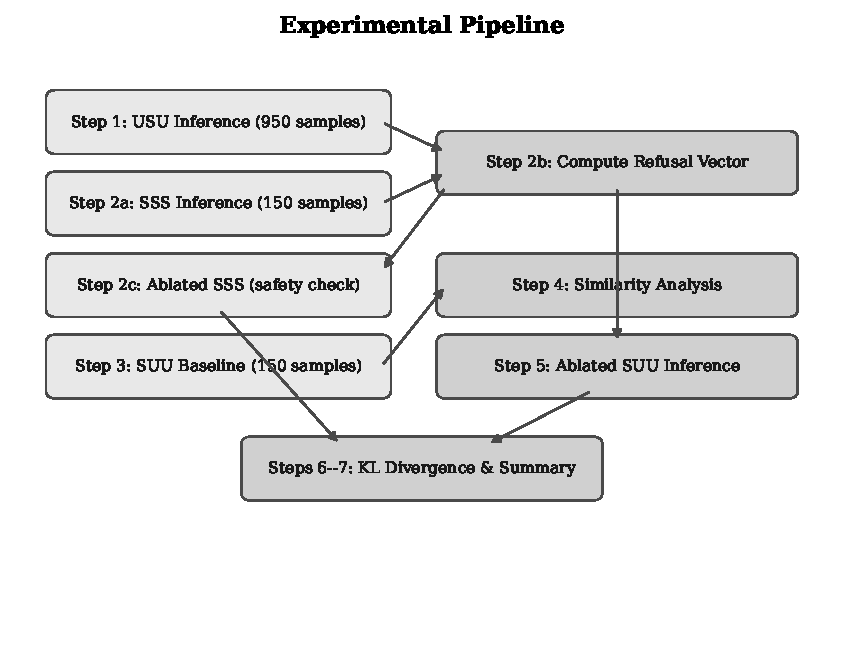
\includegraphics[width=\textwidth]{../figures/experiment_pipeline.pdf}
    \caption{Schematic of the seven-step experimental pipeline. Steps 1 and 2a provide the activations needed to compute the refusal vector in Step 2b. The vector is then applied in two directions: as a safety check on safe inputs (Step 2c) and as a jailbreak attempt on text-only unsafe inputs (Steps 3--5).}
    \label{fig:pipeline}
\end{figure}

\subsection{Step 1: USU Inference (Image-Conditioned Refusal Collection)}

We ran all 950 USU samples through the model, presenting each as its \textit{image only} (no text query). For every sample, we collected the last-token activation vector $\mathbf{h}_\ell^{(i)} \in \mathbb{R}^{d}$ at each layer $\ell \in \{13, \ldots, 31\}$ and saved them to disk. Each response was judged for refusal.

Out of 950 samples, only \textbf{10 triggered refusal} (1.05\% refusal rate). This is expected: since the text component is safe (or absent), the model has little reason to refuse. However, the low count of refused samples means the refusal vector is estimated from a small basis, which we discuss as a key limitation in Section~\ref{sec:limitations}.

\subsection{Step 2: Refusal Vector Computation}

\paragraph{Step 2a: SSS baseline activations.} We ran 150 SSS samples (safe image + safe text) through the model, again collecting last-token activations at layers 13--31. We also collected output logits at every generated token for later use in the KL divergence analysis.

\paragraph{Step 2b: Refusal vector extraction.} For each layer $\ell$, the refusal direction was computed as:
\begin{equation}
    \mathbf{d}_\ell = \frac{\bar{\mathbf{h}}_\ell^{\text{USU}} - \bar{\mathbf{h}}_\ell^{\text{SSS}}}{\left\| \bar{\mathbf{h}}_\ell^{\text{USU}} - \bar{\mathbf{h}}_\ell^{\text{SSS}} \right\|}
\end{equation}
where $\bar{\mathbf{h}}_\ell^{\text{USU}}$ is the mean activation across the 10 \textit{refused} USU samples and $\bar{\mathbf{h}}_\ell^{\text{SSS}}$ is the mean across all 150 SSS samples. The resulting unit vector $\mathbf{d}_\ell$ captures the direction in activation space that distinguishes refused image inputs from safe image inputs at layer $\ell$.

\paragraph{Step 2c: Safety check (ablated SSS).} To verify that subtracting the refusal vector does not damage safe behavior, we re-ran all 150 SSS samples with the refusal vector ablated. The ablation was implemented via forward hooks: at each layer $\ell$, the last-token hidden state $\mathbf{h}$ was modified as:
\begin{equation}
    \mathbf{h}' = \mathbf{h} - (\mathbf{h} \cdot \mathbf{d}_\ell)\, \mathbf{d}_\ell
\end{equation}
This is a standard directional ablation---it projects out the component of $\mathbf{h}$ along the refusal direction while preserving all orthogonal components. The ablated SSS refusal rate was \textbf{0.0\%}, confirming that the refusal vector does not induce false refusals on safe inputs.

\subsection{Step 3: SUU Baseline (Text-Only Unsafe Queries)}

We extracted the text queries from 150 SUU samples and ran them through the model as \textit{text-only inputs} (no image). This establishes the baseline refusal rate for unsafe text queries without any intervention.

The baseline refusal rate was \textbf{74.67\%} (112 out of 150 samples refused). This means the model correctly identifies and refuses roughly three-quarters of the unsafe text queries under normal conditions.

\subsection{Step 4: Layer-wise Similarity Analysis}

Before ablation, we measured how much the image-derived refusal vector aligns with text-only activations. For each of the 112 refused SUU samples, we computed the dot product $\mathbf{d}_\ell \cdot \mathbf{h}_\ell^{(i)}$ at every layer. A high dot product indicates that the text-only activation has a large component along the image-derived refusal direction---a necessary (but not sufficient) condition for ablation to suppress refusal.

\subsection{Step 5: Ablated SUU Inference (The Jailbreak Attempt)}

We re-ran all 150 SUU text queries through the model with the image-derived refusal vector ablated at every layer (using the same directional projection as in Step 2c). The ablated refusal rate was \textbf{54.67\%} (82 out of 150 samples). This represents a \textbf{20.0 percentage-point drop} from the 74.67\% baseline, which we report as the jailbreak success rate.

\subsection{Step 6: KL Divergence (Ablation Side-Effect Check)}

To quantify whether the ablation disturbs the model's output distribution on safe inputs, we computed the KL divergence between the original SSS logits (Step 2a) and the ablated SSS logits (Step 2c) at the \textbf{first generated token}. We restrict to the first token because subsequent tokens diverge due to autoregressive feedback from different prefixes, making token-by-token comparison uninformative beyond position 0.

For each sample $i$:
\begin{equation}
    D_{\mathrm{KL}}^{(i)} = \sum_v p_v^{(i)} \log \frac{p_v^{(i)}}{q_v^{(i)}}
\end{equation}
where $p^{(i)}$ is the softmax of the original logits and $q^{(i)}$ is the softmax of the ablated logits, both over the full vocabulary $v$.

% ──────────────────────────────────────────────────────────────────────────
\section{Results}
% ──────────────────────────────────────────────────────────────────────────

\subsection{Refusal Rates}

Table~\ref{tab:refusal} summarizes the refusal rates across all experimental conditions, and Figure~\ref{fig:refusal_rates} visualizes them.

\begin{table}[H]
\centering
\caption{Refusal rates across experimental conditions.}
\label{tab:refusal}
\begin{tabular}{llcc}
\toprule
\textbf{Condition} & \textbf{Input Type} & \textbf{Refusal Rate} & \textbf{Count} \\
\midrule
USU (baseline) & Image only (unsafe img) & 1.05\% & 10 / 950 \\
SSS (ablated, safety check) & Image + text (safe) & 0.00\% & 0 / 150 \\
SUU (baseline) & Text only (unsafe text) & 74.67\% & 112 / 150 \\
SUU (ablated) & Text only (unsafe text) & 54.67\% & 82 / 150 \\
\midrule
\textbf{Jailbreak success} ($\Delta$) & --- & \textbf{20.00\%} & \textbf{30 / 150} \\
\bottomrule
\end{tabular}
\end{table}

\begin{figure}[H]
    \centering
    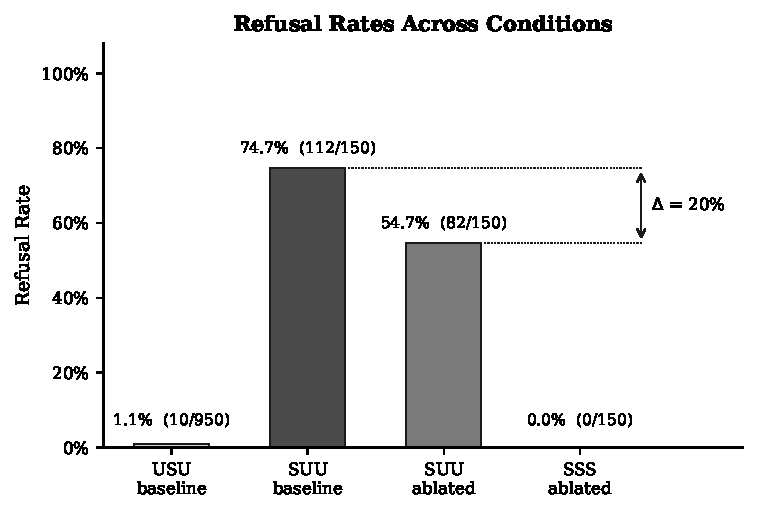
\includegraphics[width=0.85\textwidth]{../figures/refusal_rates.pdf}
    \caption{Refusal rates across experimental conditions. The arrow highlights the 20 percentage-point drop in refusal rate after ablation---the jailbreak success rate.}
    \label{fig:refusal_rates}
\end{figure}

The 20\% jailbreak success rate indicates a partial but meaningful cross-modal transfer of the refusal direction. The image-derived vector successfully flipped 30 out of 150 text-only inputs from refusal to compliance. However, the majority of inputs (82/150) continued to be refused even after ablation, suggesting that the text-modality refusal mechanism is not fully captured by the image-derived direction.

\subsection{Layer-wise Alignment}

Figure~\ref{fig:layer_dots} shows the mean dot product between the image-derived refusal vector and the text-only SUU activations across layers 13--31, and Figure~\ref{fig:layer_range} shows the full min/max range.

\begin{figure}[H]
    \centering
    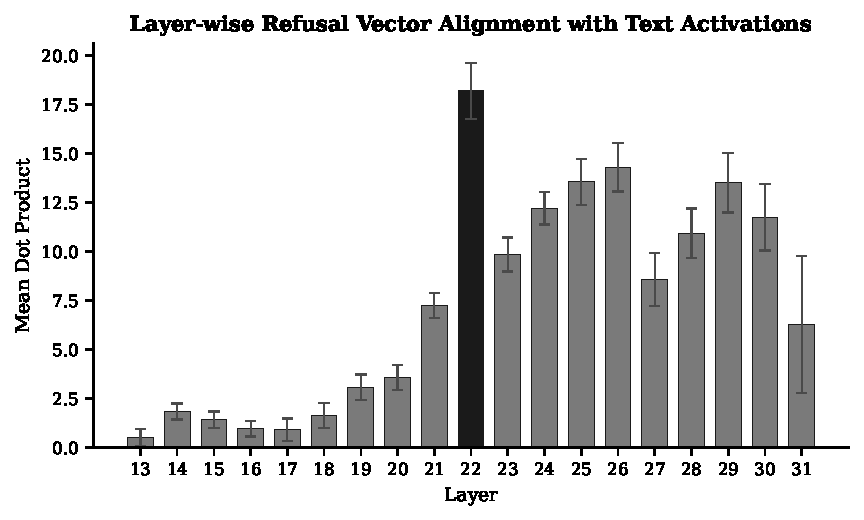
\includegraphics[width=0.85\textwidth]{../figures/layer_dot_products.pdf}
    \caption{Mean dot product between the image-derived refusal vector $\mathbf{d}_\ell$ and refused text-only (SUU) activations at each layer, with $\pm 1$ standard deviation error bars. Layer 22 shows the strongest alignment ($\mu = 18.21$).}
    \label{fig:layer_dots}
\end{figure}

\begin{figure}[H]
    \centering
    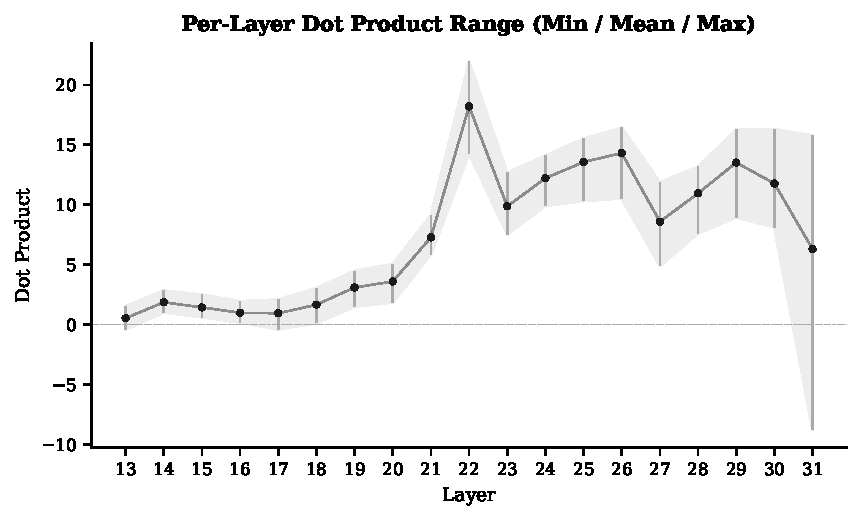
\includegraphics[width=0.85\textwidth]{../figures/layer_dot_range.pdf}
    \caption{Per-layer dot product range showing mean (points), $\pm 1$ std (dark band via error bars), and full min--max range (shaded region). The spread widens considerably in later layers (27--31), suggesting more variable alignment in the final transformer blocks.}
    \label{fig:layer_range}
\end{figure}

Key observations from the layer analysis (see also Table~\ref{tab:layers} for exact values):

\begin{itemize}[nosep]
    \item \textbf{Peak alignment at layer 22} ($\mu = 18.21$, $\sigma = 1.43$). This layer shows by far the strongest projection of text activations onto the image-derived refusal direction.
    \item \textbf{Secondary peaks at layers 25--26 and 29} ($\mu \approx 13.5$--$14.3$). These form a second cluster of high alignment in the later layers.
    \item \textbf{Early layers (13--17) show weak alignment} ($\mu < 2$). The refusal signal has not yet coalesced in these layers.
    \item \textbf{Layer 31 (final) shows high variance} ($\sigma = 3.51$, range $[-8.77, 15.77]$). Some samples have \textit{negative} dot products at this layer, meaning their activation points \textit{away} from the refusal direction. This is consistent with the model potentially ``resolving'' the refusal decision non-uniformly in the final layer.
\end{itemize}

\begin{figure}[H]
    \centering
    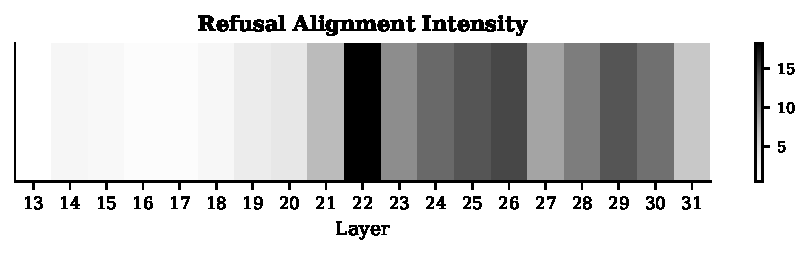
\includegraphics[width=0.85\textwidth]{../figures/layer_dot_heatmap.pdf}
    \caption{Heatmap visualization of mean dot product intensity across layers. The bright band at layer 22 corresponds to peak cross-modal refusal alignment.}
    \label{fig:heatmap}
\end{figure}

\begin{table}[H]
\centering
\caption{Layer-by-layer dot product statistics for the image-derived refusal vector projected onto refused text-only (SUU) activations.}
\label{tab:layers}
\small
\begin{tabular}{ccccc}
\toprule
\textbf{Layer} & \textbf{Mean} & \textbf{Std} & \textbf{Min} & \textbf{Max} \\
\midrule
13 & 0.52 & 0.42 & $-$0.41 & 1.52 \\
14 & 1.85 & 0.40 & 1.01 & 2.82 \\
15 & 1.42 & 0.43 & 0.61 & 2.47 \\
16 & 0.97 & 0.39 & 0.17 & 1.93 \\
17 & 0.93 & 0.57 & $-$0.41 & 2.07 \\
18 & 1.65 & 0.64 & 0.12 & 3.02 \\
19 & 3.08 & 0.65 & 1.49 & 4.46 \\
20 & 3.58 & 0.62 & 1.85 & 5.03 \\
21 & 7.27 & 0.63 & 5.85 & 9.09 \\
\textbf{22} & \textbf{18.21} & \textbf{1.43} & \textbf{14.29} & \textbf{21.92} \\
23 & 9.86 & 0.87 & 7.55 & 12.65 \\
24 & 12.21 & 0.82 & 9.91 & 14.09 \\
25 & 13.56 & 1.18 & 10.31 & 15.49 \\
26 & 14.31 & 1.24 & 10.53 & 16.41 \\
27 & 8.58 & 1.36 & 4.89 & 11.86 \\
28 & 10.95 & 1.26 & 7.61 & 13.15 \\
29 & 13.51 & 1.51 & 8.95 & 16.25 \\
30 & 11.76 & 1.70 & 8.12 & 16.28 \\
31 & 6.29 & 3.51 & $-$8.77 & 15.77 \\
\bottomrule
\end{tabular}
\end{table}

\subsection{KL Divergence}

The KL divergence between original and ablated SSS logits was extremely low (Table~\ref{tab:kl}, Figure~\ref{fig:kl}).

\begin{table}[H]
\centering
\caption{KL divergence statistics (SSS original vs.\ ablated, first generated token, $n = 150$).}
\label{tab:kl}
\begin{tabular}{lc}
\toprule
\textbf{Statistic} & \textbf{Value} \\
\midrule
Mean & 0.0195 \\
Std Dev & 0.0291 \\
Min & 0.0012 \\
Max & 0.2385 \\
\bottomrule
\end{tabular}
\end{table}

\begin{figure}[H]
    \centering
    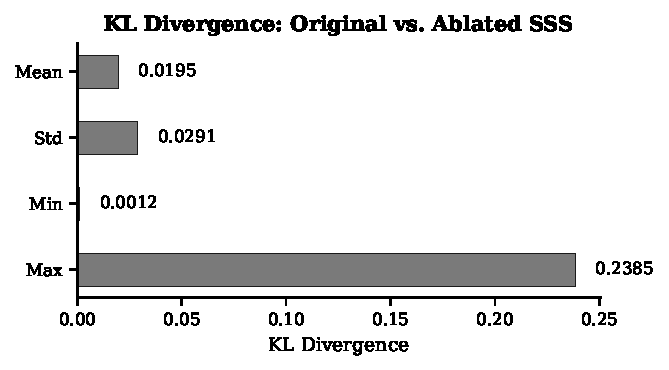
\includegraphics[width=0.7\textwidth]{../figures/kl_summary.pdf}
    \caption{Summary of KL divergence between original and ablated SSS logits. A mean of 0.02 indicates near-identical output distributions, confirming the ablation does not degrade safe behavior.}
    \label{fig:kl}
\end{figure}

A mean KL of 0.0195 is negligible in practice---it means the probability distributions over the vocabulary at the first generated token are nearly identical with and without the refusal vector ablation. Combined with the 0\% false-refusal rate on ablated SSS inputs, this confirms that the ablation procedure is \textit{safe}: it does not cause the model to refuse safe inputs or meaningfully alter its safe-input behavior.

The single outlier at $D_{\mathrm{KL}} = 0.2385$ deserves attention. While still moderate, it is an order of magnitude above the mean and suggests that for certain inputs, the refusal direction overlaps with features relevant to safe generation. Without the per-sample KL values (lost with the \texttt{results/} directory), we cannot identify which sample this was, but future reruns should flag and inspect such outliers.

It is also worth noting that the KL divergence itself is downstream of the noisy $n = 10$ refusal vector. A more precisely estimated refusal direction---one that more cleanly isolates the refusal component from unrelated variance---would likely produce an even \textit{lower} KL divergence, since less non-refusal signal would be projected out during ablation. Further studies with higher USU refusal rates are needed to confirm this.

% ──────────────────────────────────────────────────────────────────────────
\section{Discussion}
% ──────────────────────────────────────────────────────────────────────────

\subsection{Interpretation of the 20\% Jailbreak Success}

The 20\% jailbreak success rate is a positive result, but \textbf{it is critically ambiguous in its interpretation}. There are two competing explanations, and this experiment cannot distinguish between them:

\begin{enumerate}[nosep]
    \item \textbf{Partial overlap.} The image-derived and text-derived refusal directions are genuinely distinct subspaces that only partially overlap. The 20\% reflects the true degree of cross-modal sharing, and a better-estimated vector would not substantially improve the jailbreak rate.
    \item \textbf{Full overlap, noisy estimate.} The refusal direction is in fact fully shared across modalities, but our refusal vector---estimated from only $n = 10$ refused samples---is a poor approximation of the true direction. A more accurate estimate (from hundreds of refused samples) could yield a jailbreak rate far higher than 20\%, potentially approaching 100\%.
\end{enumerate}

\noindent We consider explanation (2) at least as plausible as (1), and possibly more so. With only 10 samples contributing to $\bar{\mathbf{h}}_\ell^{\text{USU}}$, the estimated mean is dominated by sampling noise. In a hidden-state space of dimension $d = 3584$ (for Qwen3.5-9B), 10 samples provide almost no statistical power to estimate a mean direction reliably. The resulting refusal vector likely captures some true refusal signal mixed with substantial noise, meaning the directional ablation only partially removes the refusal component even if the true direction would fully remove it.

\textbf{Therefore, the 20\% figure should be read as a lower bound on cross-modal transfer, not as evidence that the overlap is partial.} The true transfer rate is unknown and could be substantially higher. Resolving this ambiguity requires conducting further studies with a substantially higher USU refusal rate---by generating custom images that reliably trigger refusal, we can estimate the refusal vector from hundreds rather than tens of samples and determine whether the 20\% gap closes. Until then, no strong conclusion can be drawn about the degree of cross-modal sharing.

\subsection{The Peak at Layer 22}

The sharp peak in dot product at layer 22 (mean 18.21, compared to 14.31 at the next-highest layer 26) suggests that cross-modal refusal alignment is concentrated in a specific part of the network rather than distributed uniformly. This is reminiscent of findings in the text-only refusal literature, where refusal directions tend to be strongest in a narrow band of middle-to-late layers. The fact that the \textit{image-derived} direction shows the same localized peak when projected onto \textit{text} activations is noteworthy: it implies that layer 22 plays a privileged role in refusal processing regardless of input modality.

The high variance at layer 31 ($\sigma = 3.51$, with negative dot products for some samples) may reflect the final layer's role in ``resolving'' ambiguous cases---samples where the model is uncertain about whether to refuse might show inconsistent alignment with the refusal direction at the decision boundary.

\subsection{Limitations}
\label{sec:limitations}

\paragraph{Small refusal sample size (critical).} As discussed in Section 5.1, the refusal vector was computed from only \textbf{10 refused USU samples} out of 950 total. This is the most significant limitation of the study and the reason the 20\% result is uninterpretable as either ``partial'' or ``full'' cross-modal overlap. Every quantitative finding in this report---the jailbreak rate, the layer-wise dot products, the KL divergence---is downstream of this single noisy estimate. Until the refusal vector is re-estimated from a substantially larger sample, no strong conclusions about the \textit{degree} of cross-modal sharing can be drawn.

\textbf{Mitigation plan:} We plan to generate custom unsafe images (rather than relying on the HoliSafe dataset) to increase the number of image-conditioned refusals. By controlling the image content directly, we can engineer images that more reliably trigger refusal and obtain a larger, more representative sample for refusal vector estimation.

\paragraph{Keyword-based refusal judge.} The keyword matcher is fast and deterministic but may miss refusals expressed in unusual phrasings (e.g., ``That's not appropriate'' or simply refusing to answer without an explicit marker). It may also false-positive on responses that use refusal-like language in a compliant context (e.g., ``I can't stress enough how important this is...''). A model-based judge would be more robust but introduces its own biases and non-determinism.

\paragraph{Single model.} All results are from Qwen3.5-9B. We make no claims about generalization to other VLMs, architectures, or model scales. The cross-modal transfer rate may be higher or lower in models with different fusion architectures or safety training procedures.

\paragraph{Ablation across all layers simultaneously.} We ablated the refusal vector at all 19 layers simultaneously. This means we cannot attribute the jailbreak effect to any specific layer. The layer-wise dot product analysis (Section 4.2) provides correlational evidence for which layers matter most, but a controlled per-layer ablation study would be needed to establish causal contributions.

% ──────────────────────────────────────────────────────────────────────────
\section{Conclusion and Next Steps}
% ──────────────────────────────────────────────────────────────────────────

We find that an image-derived refusal vector achieves a \textbf{20\% jailbreak success rate} when applied to text-only unsafe inputs on Qwen3.5-9B, reducing the text refusal rate from 74.67\% to 54.67\%. The ablation introduces negligible distortion to safe outputs (mean KL divergence = 0.02, 0\% false refusal on safe inputs). Cross-modal alignment peaks sharply at layer 22, suggesting localized rather than diffuse sharing of refusal representations across modalities.

Crucially, the 20\% figure is a \textbf{lower bound}, not a point estimate of cross-modal overlap. Because the refusal vector was estimated from only 10 samples, it is likely a noisy approximation of the true refusal direction. The true cross-modal transfer rate could be substantially higher---possibly indicating full geometric overlap between image and text refusal subspaces. \textbf{Further studies with substantially higher USU refusal rates are essential} to determine (1) whether the 20\% gap was simply an artifact of the noisy refusal vector and (2) whether a cleaner refusal direction would yield even lower KL divergence on safe inputs. Until the refusal vector can be re-estimated from a much larger sample, the degree of cross-modal sharing remains an open question. Immediate next steps include:

\begin{enumerate}[nosep]
    \item \textbf{Custom image generation.} Generate unsafe images programmatically to increase the refusal sample pool and obtain a more robust refusal vector estimate. This is the single most important follow-up: every quantitative conclusion in this report is downstream of the $n = 10$ estimate, and a larger sample would either confirm or substantially revise the 20\% figure.
    \item \textbf{Reverse-causality test via refusal vector addition.} Rather than subtracting the refusal vector from unsafe text inputs, \textit{add} it to safe text inputs and measure whether the model begins refusing benign queries. If adding the image-derived direction induces text refusal, this provides stronger causal evidence that the direction genuinely encodes cross-modal refusal, rather than merely correlating with it.
    \item \textbf{Model-based judge.} Replace or supplement the keyword matcher with an LLM-based refusal judge for more nuanced classification of refusal behavior.
\end{enumerate}

\end{document}
